\documentclass[12pt,a4paper,table]{article}

\usepackage[a4paper,
            tmargin=2cm,
            bmargin=2cm,
            lmargin=2cm,
            rmargin=2cm,
            bindingoffset=0cm]{geometry}

\usepackage{lmodern}
\usepackage[T1]{polski}
\usepackage[utf8]{inputenc}
\usepackage{tocloft}
\usepackage{hyperref}
\usepackage{amsmath}
\usepackage{listings}
\usepackage{graphicx}
\usepackage{subfig}
\usepackage{float}
\usepackage{booktabs}

\hypersetup{
    colorlinks,
    citecolor=black,
    filecolor=black,
    linkcolor=black,
    urlcolor=black
}

\newtheorem{definition}{Def}


\begin{document}
    \title {
        Symulacja Systemów i Modelowanie \\
        Raport 2 \\
        Wariant Flocking Algorithm zakładający omijanie losowo generowanych przeszkód

    }

    \author{
        Adam Staniszewski \\
        Dariusz Królicki
    }

    \date{\today}

    \maketitle

    \tableofcontents
    \newpage

    \section{Zmiany kosmetyczne względem poprzedniej wersji projektu}
    Wraz z nową iteracją projektu przygotowane zostały dwie zmiany, które nie są znaczące dla przygotowywanych funkcjonalności, jednak zwiększają czytelność i ogólną estetykę kodu. 

    Po pierwsze, klasa \textbf{Obstacle} używa teraz dekoratora \textbf{dataclass} - od teraz służy ona jedynie do przechowywania danych i nie posiada własnych metod.

    \raggedright
    \vskip
    \begin{lstlisting}[language=Python]
    @dataclass
    class Obstacle:
        """
        Attributes:
            x: x-coordinate of the obstacle's center
            y: y-coordinate of the obstacle's center
        """
        def __init__(self, x, y, radius, screen):
            self.position = (x, y)
            self.screen = screen
            self.radius = radius
    \end{lstlisting}
    
    Po drugie, do projektu został dodany moduł \textbf{pylint\_runner}, który pomaga w dostosowywaniu kodu do standardu PEP 8.

    \raggedright
    \vskip
    \begin{lstlisting}[language=Python]
    def run_pylint_on_folder(folder_path):
        for root, _, files in os.walk(folder_path):
            for file in files:
                if file.endswith(".py"):
                    file_path = os.path.join(root, file)
                    print(f"Running pylint on: {file_path}")
                    os.system(f"pylint {file_path}")
    \end{lstlisting}
    
    \section{Nowe funkcjonalności}
    \subsection{Sposób generowania przeszkód}
    Przeszkody są od teraz generowane losowo. Współrzędne są wybierane losowo przy użyciu rozkładu jednostajnego, z zakresu obejmującego rozdzielczość ekranu symulacji.
    \raggedright
    \vskip
    \begin{lstlisting}[language=Python]
    min_x = 0
    max_x = 1366
    min_y = 0
    max_y = 768
    random_positions = [
    (random.randint(min_x, max_x),  
    random.randint(min_y, max_y))  for _ in range(10)
    ]
    \end{lstlisting}
    
    \subsection{Kontrola symulacji}
    Symulacja może być teraz resetowana przy użyciu odpowiedniego klawisza - pomaga to przy testowaniu.
    \raggedright
    \vskip
    \begin{lstlisting}[language=Python]
    def check_keys(self):
        self.keys = pygame.key.get_pressed()
        if self.keys[pygame.K_r]:
            current_time = pygame.time.get_ticks()
            if current_time - self.reset_cooldown > self.last_reset_time:
                self.reset_simulation()
                self.last_reset_time = current_time


    def reset_simulation(self):
        self.flock.clear()
        self.obstacles.clear()

        self.start()
    \end{lstlisting}

    Zmienne \textbf{reset\_cooldown} i \textbf{last\_reset\_time} należą do klasy \textbf{Environment}. Pierwsza z nich określa, kiedy ostatnio wykonany był reset symulacji, druga to czas między kolejnymi możliwymi resetami (bazowo 1 sekunda). Zapobiega to sytuacji, w której jedno naciśnięcie klawisza wielokrotnie zresetuje symulację.
    
    \subsection{Interakcje między obiektami}
    Prace nad nową wersją projektu skupiły się na interkacji ptaków z przeszkodami. Z tego względu paramtetr \textbf{perception\_radius} został rozdzielony na dwa. Jeden z nich określa zasięg widzenia innych ptaków, a drugi przeszkód.

    \begin{lstlisting}[language=Python]
    self.perception_radius_flock: int = perception_radius[0]
    self.perception_radius_obstacle: int = perception_radius[1]
    \end{lstlisting}

    \textbf{Perception radius} jest teraz przekazywany do konstruktora klasy \textbf{Bird} jako lista.

    Klasa \textbf{Bird} została rozszerzona o cztery nowe wartości:

    \begin{enumerate}
        \item \textbf{has\_neighbors} - bool;
        \item \textbf{approaching\_obstacle} - bool;
        \item \textbf{last\_projection\_time} - int;
        \item \textbf{projection\_cooldown} - int;
    \end{enumerate}

    \begin{lstlisting}[language=Python]
    self.has_neighbors: bool = False
    self.approaching_obstacle: bool = False
    self.last_projection_time = 0
    self.projection_cooldown: float = 0.1
    \end{lstlisting}

    Flaga \textbf{has\_neighbors} służy do sygnalizowania, że w perception radius danego osobnika znajduje się inny. Ustawienie wartości na \textbf{True} powoduje zmianę koloru obrysu perception radius.    

    \begin{figure}[H]
        \centering
        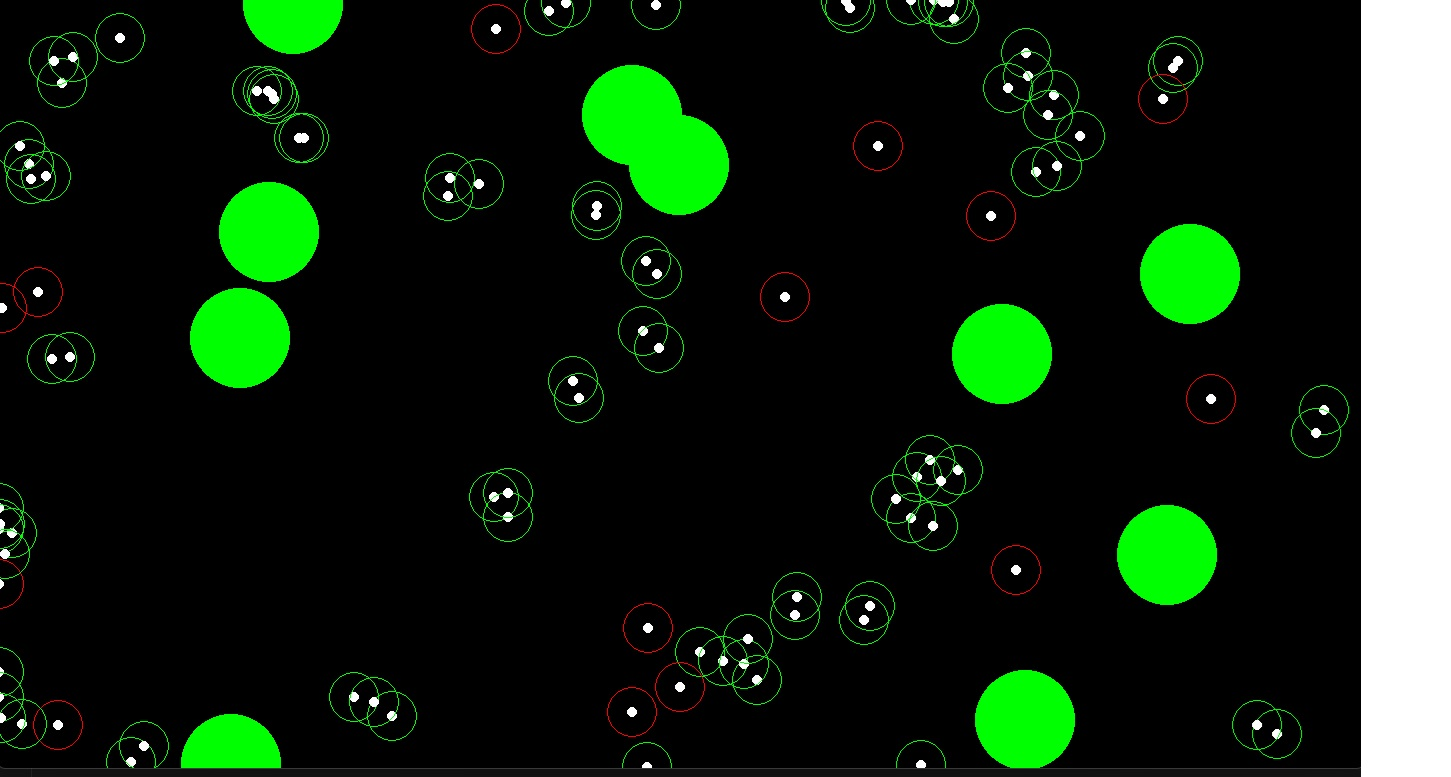
\includegraphics[width=1\textwidth]{images/perception_radius.jpg}
        \caption{Osobniki z czerwonym okręgiem wokół nie posiadają sąsiadów.}
        \label{fig:example}
    \end{figure}

    Pozostałe parametry są wykorzystywane przez nową metodę - \textbf{dodge\_obstacles}.

    \begin{figure}[H]
        \centering
        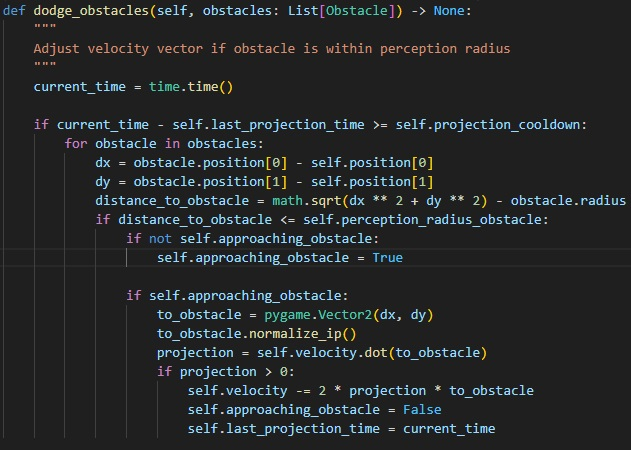
\includegraphics[width=1\textwidth]{images/kod1.jpg}
        \caption{Metoda \textbf{dodge\_obstacles}, Sposób formatowania kodu wymusił wstawienie screenshota.}
        \label{fig:example}
    \end{figure}

    Metoda sprawdza odległość między osobnikiem, a przeszkodami. Jeśli odległość od przeszkody jest mniejsza niż odpowiedni perception radius, to obliczony zostanie \textbf{projection}, który wskaże kierunek ruchu osobnika względem przeszkody. Jeśli osobnik zmierza ku przeszkodzie, to wektor jego ruchu jest modyfikowany tak, aby uniknąć kolizji.
    Wyjątek stanowi sytuacji, w której od ostatniej transformacji wektora minęło za mało czasu - gdyby nie to zabezpieczenie, to na granicy perception radius osobnik zatrzymałbym się, ciągle korygując tor lotu.
    W przypadku zblizającej się kolizji, perception\_radius\_obstacle zmienia kolor z zielonego na czerwony.

    \begin{figure}[H]
        \centering
        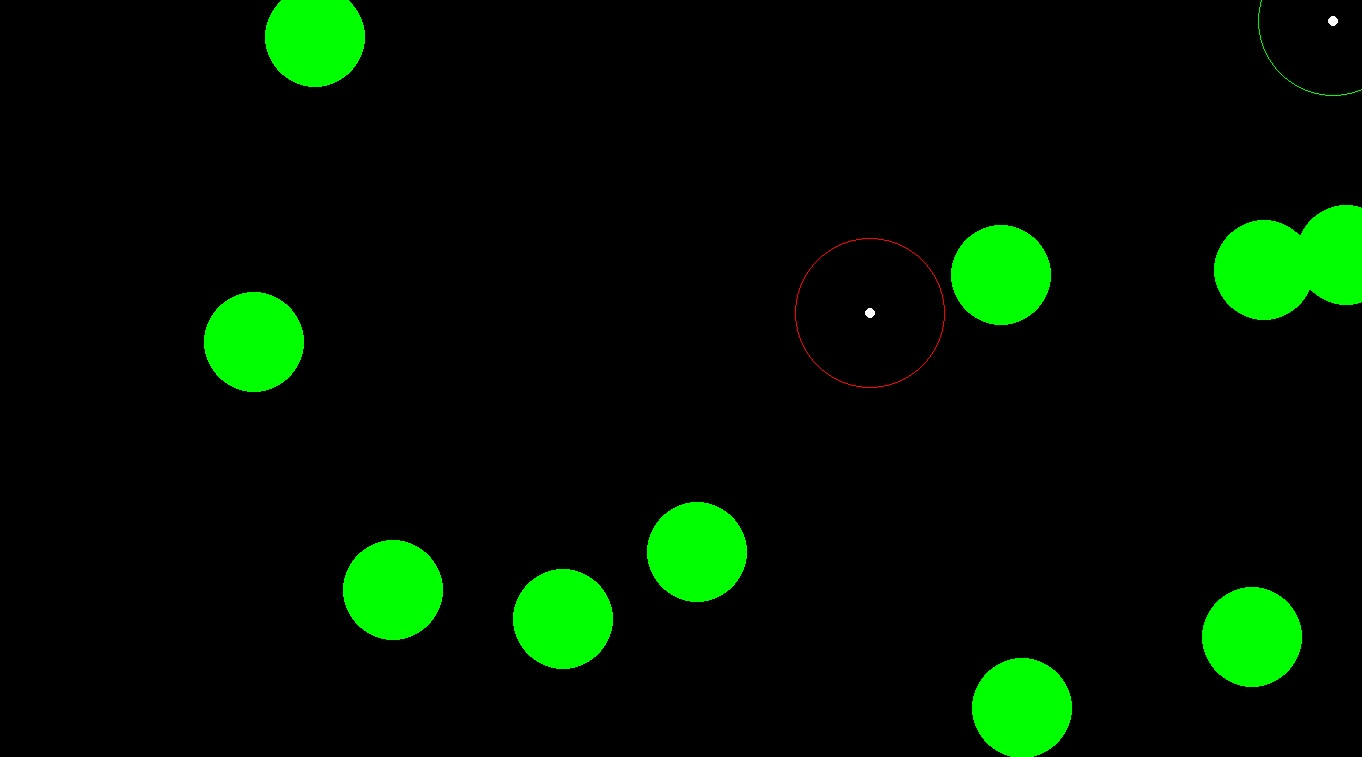
\includegraphics[width=1\textwidth]{images/perception_radius2.jpg}
        \caption{Osobniki z czerwonym okręgiem wokół są niebezpiecznie blisko przeszkody.}
        \label{fig:example}
    \end{figure}

    \section{Kolejne planowane etapy rozwoju projektu}
    Na myśli przychodzą dwie oczywiste modyfikacje. Po pierwsze można zastasować sposób obliczania odległości niewykorzystujący relatywnie kosztownego pierwiastkowania, Po drugie, można rozpatrzyć zmodyfikowanie funkcji odpowiedzialnej za ominajnie przeszkód, tak aby proces był bardziej płyny, dzięki czemu wyeliminowana zostanie potrzeba korzystania ze zmiennych \textbf{last\_projection\_time} i \textbf{projection\_cooldown}.

    \vspace{2em}

    Kolejne iteracje projektu można śledzić pod adresem:
    \url{https://github.com/StaniszewskiA/SSIM-Proj}

\end{document}